\documentclass[11pt]{article}
\usepackage[margin=1in]{geometry}
\usepackage{amsmath,amssymb}
\usepackage{booktabs}
\usepackage{graphicx}
\usepackage{hyperref}
\usepackage{xcolor}
\usepackage[numbers]{natbib}
\usepackage{enumitem}
\usepackage{caption}
\usepackage{subcaption}
\setlist{nosep}

\graphicspath{{../experiments/results/}}

\newcommand{\eps}{\varepsilon}
\newcommand{\epspert}{\eps_\mathrm{pert}}
\newcommand{\rhogeo}{\rho_\mathrm{geo}}
\newcommand{\rhohol}{\rho_\mathrm{hol}}
\newcommand{\Gr}{\mathrm{Gr}}

\title{Separating signal from noise in geometric
  cross-sensor metrics: a pre-registered case study}
\author{Elliot Tower\textsuperscript{1}}
\date{}

\begin{document}
\maketitle

\noindent\textsuperscript{1}Independent Researcher\\
\noindent Correspondence: \href{mailto:elliot@elliottower.com}{elliot@elliottower.com}

\bigskip

% ================================================================
\begin{abstract}
Grassmannian geodesic distance between PCA subspaces offers a
parameter-free measure of cross-sensor consistency: when multiple
sensors observe the same latent process, their estimated subspaces
should align, and divergence signals genuine disagreement about the
underlying signal.  Validating this metric, however, requires care.
We present a case study in which a naive single-parameter simulation
design confounded observation noise with embedding perturbation,
producing spurious positive results that survived standard
significance testing.  Through four pre-registered iterations---each
corrected after negative controls exposed a specific flaw---we
developed a two-axis experimental design that cleanly separates
noise from perturbation.  The resulting degradation curve
characterizes the operating regime: at low noise
($\sigma = 1.0$), geodesic distance reliably detects cross-sensor
perturbation (median $\rhogeo = 0.52$, 95\% CI excludes zero,
62\% per-seed detection); at high noise ($\sigma = 4.5$), the
signal is fully attenuated (median $\rhogeo = 0.15$, 0\%
per-seed detection).  We also report a negative result for loop
holonomy, a candidate severity metric: it is genuinely
non-monotone in perturbation magnitude, functioning as a
saturating onset detector sensitive to presence but insensitive
to severity.  The
two-axis design principle and degradation-curve methodology
transfer to any setting where geometric cross-sensor metrics
require validation.
\end{abstract}

\noindent\textbf{Keywords:}
Grassmannian, geodesic distance, PCA subspaces, cross-sensor
consistency, pre-registration, negative controls, simulation design,
metric validation

% ================================================================
\section{Introduction}
\label{sec:intro}

When multiple sensors observe the same latent process, a natural
question arises: do their measurements agree?  Agreement at the
level of summary statistics (means, variances) can mask structural
disagreement about which directions in feature space carry signal.
Grassmannian geodesic distance---the arc length between subspaces
estimated by PCA---captures this directional information without
learned parameters, offering a geometric measure of cross-sensor
consistency~\citep{edelman1998geometry, chikuse2003statistics}.

The appeal is clear: a single number quantifying how much two
sensors' measurement bases have diverged, computable from data
alone.  The difficulty is validation.  On real multi-sensor data,
ground truth is unavailable---we cannot directly observe whether a
large geodesic distance reflects genuine inconsistency or
measurement noise.  Simulation studies fill this gap, but they
introduce a subtler problem: the simulation design itself can
confound the effects it aims to isolate.

This paper documents such a confound and the iterative process that
uncovered it.  We began with a single-parameter design in which one
variable $\eps$ simultaneously controlled observation noise and
cross-sensor embedding perturbation.  Under this design, geodesic
distance increased monotonically with $\eps$---an apparently clean
signal.  Negative controls revealed the truth: the monotonicity was
driven primarily by noise scaling.  Identical
sensors (no embedding divergence) produced \emph{stronger}
monotonicity than genuinely different sensors, because the noise
ramp dominated the geodesic metric.

Correcting this required separating the two axes: observation noise
$\sigma$ (held constant within each experimental sweep) and
embedding perturbation $\epspert$ (varied independently).  The
separation was not obvious from the initial design.  It emerged
through four pre-registered iterations (Section~\ref{sec:confound}),
each frozen under a commit SHA before any confirmatory data was
generated~\citep{nosek2018preregistration}.

The resulting experiment (Section~\ref{sec:results}) yields three
contributions:

\begin{enumerate}
  \item A \textbf{two-axis design principle} for validating
    geometric cross-sensor metrics, applicable beyond the specific
    simulation studied here.
  \item A \textbf{degradation curve} characterizing the
    operating-regime boundary: the noise level at which geodesic
    distance ceases to reliably detect perturbation.
  \item A \textbf{negative result} for loop holonomy: the composed
    parallel transport around a sensor loop is non-monotone in
    perturbation, confirmed by power analysis as intrinsic to the
    metric.
\end{enumerate}

\paragraph{Related work.}
Grassmannian geometry underlies subspace comparison in signal
processing~\citep{edelman1998geometry}, with principal angles
providing the canonical distance~\citep{golub1973numerical,
ye2016schubert}.  Computational aspects are surveyed
by~\citet{bendokat2024grassmann}.  In applied settings,
cross-site harmonization methods such as
ComBat~\citep{johnson2007adjusting} and its neuroimaging
extensions~\citep{fortin2018harmonization} address batch effects
through parametric adjustments.  Geometric approaches operate
on the subspaces themselves.  The pre-registration
methodology follows~\citet{nosek2018preregistration};
\citet{simmons2011false} document the risks of undisclosed
analytic flexibility that pre-registration mitigates.

% ================================================================
\section{The confound discovery}
\label{sec:confound}

This section traces the four design iterations that preceded the
confirmatory experiment.  Each iteration discovered a flaw through
pre-registered controls, motivating a redesign.  We present them
chronologically because the sequence itself illustrates how
confounds hide in apparently reasonable designs.

\subsection{Versions 1--2: The wrong null and the wrong signal}
\label{sec:v1v2}

The initial design simulated three sensors in $\mathbb{R}^{100}$
observing a shared $k$-dimensional latent signal ($k = 3$) through
sensor-specific linear embeddings.  A single parameter $\eps \in
[0, 1]$ controlled the decoherence level, simultaneously
scaling observation noise ($\sigma = 1.0 + 3.5\eps$) and
sensor-specific embedding perturbation ($U_s(\eps) =
\mathrm{QR}(U_\mathrm{base} + \eps \cdot 1.5 \cdot P_s)$, where
$P_s$ is a random perturbation matrix unique to each sensor).

Two problems emerged before any confirmatory run.  First, the
permutation null permuted rows within each sensor, then recomputed
PCA subspaces.  Row permutation does not change the covariance
matrix, so PCA returns identical subspaces regardless of the
permutation.  The null distribution collapsed to a single point
(empirical standard deviation: $0.000$), making the test trivially
significant.  A pool-and-resplit null replaced it.

Second, the three sensors differed only in additive noise scaling,
not in embedding direction.  The geodesic metric responded to
distributional differences (different variance patterns), missing
genuine geometric disagreement about the latent signal entirely.
A redesign introduced sensor-specific embedding perturbations so
that at $\eps = 0$ all sensors share the same measurement basis,
and at $\eps > 0$ each sensor's basis tilts in a different
direction.

\subsection{Version 3: The single-parameter confound}
\label{sec:v3}

The redesigned data model (version~3) appeared sound: genuinely
different embeddings, a functional null, controlled signal
strength.  Five seeds confirmed the geodesic metric's monotonicity
(Spearman $\rho > 0.4$ in 4 of 5 seeds).  A deeper analysis,
however, revealed two problems.

The composed parallel transport around the three-sensor
loop---a candidate severity metric---showed Spearman $\rho$
between $0.01$ and $0.40$ across seeds (none significant at
$p < 0.05$), even though pairwise edge geodesics were monotone
($\rho \approx 0.5$).  The loop composition introduced
cancellations that destroyed the signal.  A power analysis over
sample sizes $N \in \{200, 500, 1000, 2000\}$ confirmed this is
intrinsic to the metric: Spearman $\rho$ plateaued well below
$+1$ and confidence bands did not narrow.

The definitive failure, however, came from a negative control.
Three sensors with \emph{identical} embedding perturbation
($P_0 = P_1 = P_2$, no geometric inconsistency) should produce
near-zero differential signal ($\Delta\rho =
\rho_\mathrm{edge} - \rho_\mathrm{loop} \approx 0$).  Instead,
the negative control produced $\Delta\rho \approx
+0.60$---\emph{larger} than the $\Delta\rho \approx +0.35$
observed under genuine inconsistency.

The mechanism: when all sensors share the same embedding, the
geodesic metric tracks observation noise scaling ($\sigma = 1.0 +
3.5\eps$) with near-perfect monotonicity ($\rho \approx 0.96$),
because increasing noise degrades PCA subspace estimation
symmetrically across sensors.  Genuine embedding perturbation
\emph{disrupts} this clean noise-driven monotonicity, producing a
weaker correlation.  The single-parameter design made
every downstream metric a proxy for noise scaling alone.

\subsection{Version 4: The two-axis design}
\label{sec:v4}

The fix separates the single $\eps$ into two orthogonal axes
(Figure~\ref{fig:schematic}):

\begin{itemize}
  \item \textbf{Embedding perturbation} $\epspert \in [0, 1]$
    controls cross-sensor divergence only: $U_s(\epspert) =
    \mathrm{QR}(U_\mathrm{base} + \epspert \cdot 1.5 \cdot P_s)$.
  \item \textbf{Observation noise} $\sigma$ is held constant within
    each experimental sweep.
\end{itemize}

Independence of the generative axes was verified: sensor embeddings
depend only on $\epspert$, observation noise depends only on
$\sigma$, and no parameter is shared.  A known measurement-level
interaction remains: noise degrades PCA subspace estimation, which
attenuates the perturbation signal at high $\sigma$.  This is
expected (noise masks signal), a measurement-level interaction
distinct from the generative-model confound in version~3.
The noise grid documents this attenuation explicitly.

The primary endpoint sweeps $\epspert$ at each of four fixed noise
levels ($\sigma \in \{1.0, 2.0, 3.0, 4.5\}$), with the
confirmatory test at $\sigma = 1.0$ (pre-committed as the most
favorable operating point).  Separate seed pools (50 primary, 50
negative control, 50 noise-axis control) ensure no data reuse.

\begin{figure}[t]
  \centering
  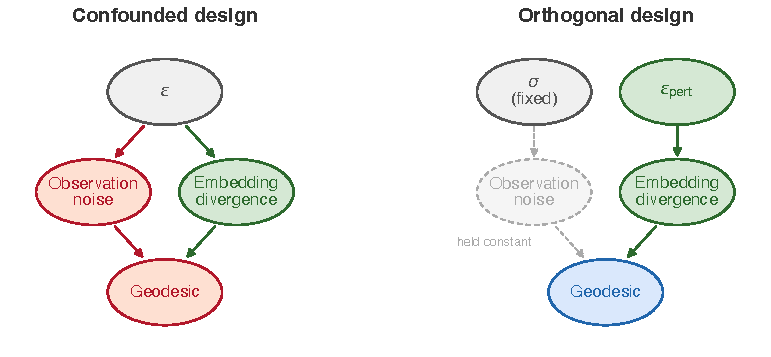
\includegraphics[width=\linewidth]{b2_confound_schematic.pdf}
  \caption{Experimental design comparison.
    \textbf{Left (confounded):} a single parameter $\eps$
    drives both observation noise and embedding perturbation,
    making the geodesic metric a proxy for noise scaling.
    \textbf{Right (orthogonal):} observation noise $\sigma$ is
    held constant (dashed), and only
    $\epspert$ varies, isolating the perturbation signal.}
  \label{fig:schematic}
\end{figure}

% ================================================================
\section{Methods}
\label{sec:methods}

\subsection{Data model}

Three sensors observe a shared latent process in
$\mathbb{R}^{100}$.  The latent data comprise $N = 200$ samples
per class (two classes) drawn from $\mathbb{R}^3$ with class
signal scaled by $\lambda = 5.0$.  Each sensor projects through
$U_s(\epspert) = \mathrm{QR}(U_\mathrm{base} + \epspert \cdot 1.5
\cdot P_s)$, where $U_\mathrm{base} \in \mathbb{R}^{100 \times 3}$
is a shared base embedding and $P_s \in \mathbb{R}^{100 \times 3}$
is a sensor-specific perturbation matrix.  Observations are
$X_s = Z \cdot U_s^\top + \mathcal{N}(0, \sigma^2 I)$.

At $\epspert = 0$, all sensors share $U_\mathrm{base}$: no
cross-sensor inconsistency exists.  At $\epspert > 0$, each
sensor's measurement basis tilts in a different direction,
creating genuine geometric inconsistency detectable on the
Grassmannian.

\subsection{Grassmannian geodesic distance}

For each sensor, PCA extracts the top-$k$ subspace ($k = 3$) from
the observation matrix.  Two subspaces $\mathcal{U},
\mathcal{V} \in \Gr(k, d)$ are compared via the geodesic
distance~\citep{ye2016schubert}:
\begin{equation}
  d_{\Gr}(\mathcal{U}, \mathcal{V}) =
    \|\boldsymbol{\theta}\|_2
    = \sqrt{\theta_1^2 + \cdots + \theta_k^2},
  \label{eq:geodesic}
\end{equation}
where $\theta_1, \ldots, \theta_k$ are the principal angles between
$\mathcal{U}$ and $\mathcal{V}$, computed via the SVD of
$U^\top V$~\citep{golub1973numerical}.
The mean of all three pairwise geodesic distances serves as the
per-step summary statistic.

\subsection{Loop holonomy}

Parallel transport around the sensor loop $0 \to 1 \to 2 \to 0$
is computed as $T = U_0^\top U_1 \cdot U_1^\top U_2 \cdot
U_2^\top U_0$, where $U_s$ are the $d \times k$ PCA basis
matrices~\citep{absil2008optimization, bendokat2024grassmann}.
The holonomy is $\|I_k - T\|_F$, measuring the failure of a vector
to return to itself after transport around the loop.

\subsection{Statistical framework}

\textbf{Primary statistic.}  For each seed at each fixed noise
level, compute $\rhogeo = \mathrm{Spearman}(\text{mean geodesic},
\, \epspert)$ over the 20-step sweep $\epspert \in [0, 1]$.

\textbf{Aggregate inference.}  The median $\rhogeo$ across 50
seeds and its 95\% bootstrap confidence interval
\citep{efron1979bootstrap} (10{,}000 resamples, bootstrap RNG
seed~$= 42$) constitute the primary summary.  The confirmatory
test at $\sigma = 1.0$ is confirmed if the CI excludes zero
($\alpha = 0.05$, single test, no multiplicity correction).

\textbf{Per-seed inference.}  Each seed's $p$-value from the
Spearman test is corrected within each noise level using
Benjamini--Hochberg FDR at $\alpha =
0.05$~\citep{benjamini1995controlling}.  The fraction of
significant seeds characterizes individual-seed reliability.

\textbf{Negative control.}  Three sensors with identical
perturbation ($P_0 = P_1 = P_2$) at each noise level; the
bootstrap CI must include zero.

\textbf{Noise-axis control.}  Sweep $\sigma$ from 1.0 to 4.5
(20 steps) at $\epspert = 0$ (no perturbation).  The strongly
positive $\rhogeo$ expected here documents the nuisance axis
explicitly.

\textbf{Degradation curve.}  Spearman correlation of median
$\rhogeo$ across the four noise levels.

\subsection{Software}

All experiments were implemented in Python~3.11 using NumPy~1.26,
SciPy~1.12 (for Spearman correlation and SVD), and
Matplotlib~3.8 (for figures).  Bootstrap confidence intervals used
the percentile method with 10{,}000 resamples.  No machine learning
libraries or GPU computation were required.

\subsection{Pre-registration protocol}

All parameters, seed assignments, and statistical procedures were
frozen under commit SHA \texttt{a792e25} before any confirmatory
seeds were generated.  Sanity seeds (10, used for parameter
calibration) were excluded from the confirmatory analysis.
Primary, negative control, and noise-axis control each used 50
non-overlapping seeds.  The full pre-registration document and
deviation log are reproduced in Appendix~\ref{app:deviations}.

% ================================================================
\section{Results}
\label{sec:results}

\subsection{Confirmatory test ($\sigma = 1.0$)}

At the pre-committed most-favorable noise level, the median
$\rhogeo$ across 50 primary seeds was $0.518$ (95\% CI: $[0.462,
0.576]$), excluding zero.  The negative control median was $0.050$
($[-0.065, 0.137]$), including zero as expected
(Figure~\ref{fig:degradation}a).

\subsection{Degradation curve}

Detection strength decreased monotonically with noise level
(Table~\ref{tab:degradation}, Figure~\ref{fig:degradation}).  The
aggregate CI excluded zero at all four levels, but per-seed
detection power collapsed rapidly: 62\% at $\sigma = 1.0$, 20\%
at $\sigma = 2.0$, 2\% at $\sigma = 3.0$, and 0\% at
$\sigma = 4.5$ (Figure~\ref{fig:degradation}b).

\begin{table}[t]
\centering
\caption{Degradation of geodesic detection across noise levels.
  Aggregate CI excludes zero at all levels, but per-seed power
  collapses above $\sigma \approx 2$.  The across-level Spearman
  correlation is $-1.0$, though this is guaranteed for any
  monotone 4-point sequence; per-level CIs and detection rates
  are the substantive findings.}
\label{tab:degradation}
\begin{tabular}{@{}ccccc@{}}
\toprule
$\sigma$ & Median $\rhogeo$ & 95\% CI & Excl.\ 0? & BH sig.\ (\%) \\
\midrule
1.0 & 0.518 & $[0.462, 0.576]$ & Yes & 31/50 (62\%) \\
2.0 & 0.438 & $[0.389, 0.495]$ & Yes & 10/50 (20\%) \\
3.0 & 0.325 & $[0.284, 0.410]$ & Yes & \phantom{0}1/50 \phantom{0}(2\%) \\
4.5 & 0.153 & $[0.077, 0.198]$ & Yes & \phantom{0}0/50 \phantom{0}(0\%) \\
\bottomrule
\end{tabular}
\end{table}

The distinction between aggregate and per-seed significance is
important.  Pooling 50 seeds provides sufficient power to detect a
small residual signal even at $\sigma = 4.5$, but no individual
seed at that noise level achieves significance after BH correction.
For practical deployment, the per-seed rate is the relevant measure:
a single dataset from a single experiment must stand on its own.
By this criterion, the practical operating boundary lies near
$\sigma \approx 2$, where per-seed power drops below 50\%.

\begin{figure}[t]
  \centering
  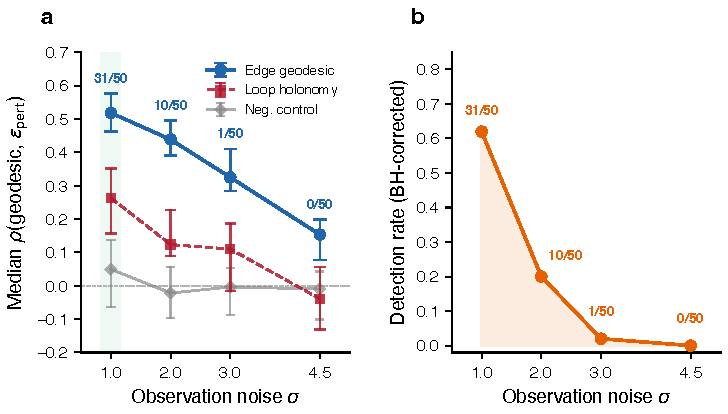
\includegraphics[width=\linewidth]{b2_degradation_curve.pdf}
  \caption{Degradation curve.
    \textbf{(a)}~Median $\rhogeo$ vs.\ observation noise $\sigma$
    for primary seeds (blue), loop holonomy (red, dashed), and
    negative control (gray).  Error bars show bootstrap 95\% CIs.
    Annotations above each point show BH-significant seed counts.
    Green band marks the confirmatory anchor at $\sigma = 1.0$.
    \textbf{(b)}~Per-seed BH detection rate.  Detection collapses
    from 62\% at $\sigma = 1.0$ to 0\% at $\sigma = 4.5$.}
  \label{fig:degradation}
\end{figure}

\subsection{Negative controls}

At all four noise levels, the negative control (identical
perturbation) produced median $\rhogeo$ with bootstrap CIs
including zero: $0.050$ at $\sigma = 1.0$, $-0.022$ at
$\sigma = 2.0$, $-0.004$ at $\sigma = 3.0$, and $-0.010$ at
$\sigma = 4.5$.  The two-axis design eliminates the spurious
signal that contaminated the single-parameter design
(Section~\ref{sec:v3}).

\subsection{Noise-axis control}

Sweeping $\sigma$ at $\epspert = 0$ yielded median $\rhogeo =
0.966$ ($[0.958, 0.973]$; Figure~\ref{fig:noiseaxis}),
confirming that geodesic distance is highly sensitive to
observation noise when noise varies.  This characterizes the
nuisance axis: the very effect that confounded the single-parameter
design is documented and accounted for by holding $\sigma$ fixed
in the primary endpoint.

\begin{figure}[t]
  \centering
  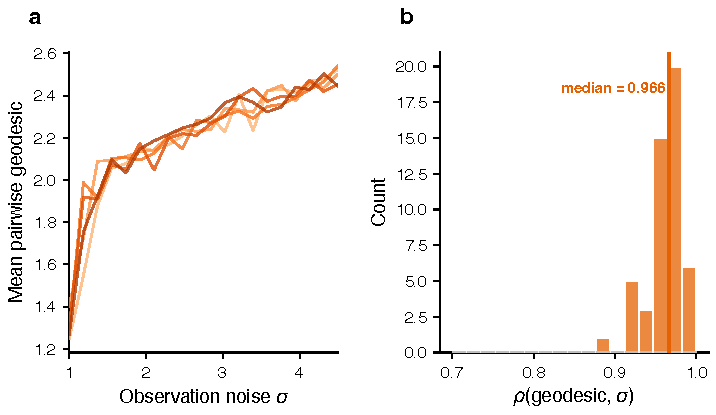
\includegraphics[width=\linewidth]{b2_noise_axis_control.pdf}
  \caption{Noise-axis control ($\epspert = 0$, no perturbation).
    \textbf{(a)}~Geodesic distance vs.\ $\sigma$ for 5 seeds,
    showing the strong monotonic relationship between noise and
    geodesic distance that the two-axis design holds constant.
    \textbf{(b)}~Distribution of $\rhogeo$ across 50 seeds
    (median $= 0.966$), confirming the nuisance axis is
    characterized.}
  \label{fig:noiseaxis}
\end{figure}

\subsection{Seed trajectories at $\sigma = 1.0$}

Figure~\ref{fig:trajectories} shows the raw geodesic-vs.-$\epspert$
curves for individual seeds at the confirmatory noise level.
Primary seeds (blue) show a consistent upward trend; negative
control seeds (gray, dashed) fluctuate around a flat baseline.
The $\rhogeo$ distribution (Figure~\ref{fig:trajectories}b)
confirms the separation: primary seeds cluster around $\rho
\approx 0.5$, while negative control seeds center near zero.

\begin{figure}[t]
  \centering
  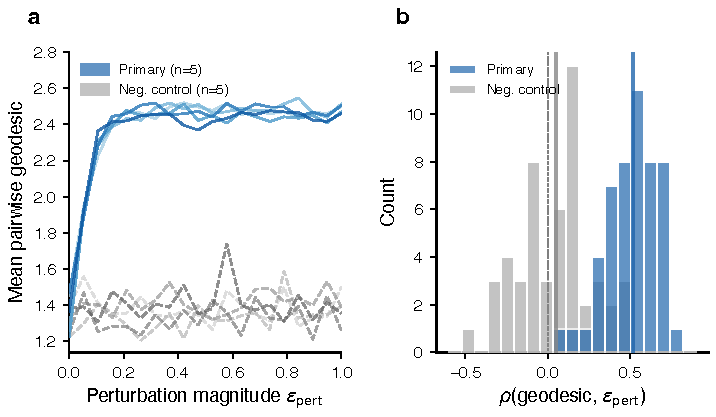
\includegraphics[width=\linewidth]{b2_seed_trajectories.pdf}
  \caption{Seed trajectories at $\sigma = 1.0$.
    \textbf{(a)}~Raw mean pairwise geodesic distance vs.\
    $\epspert$ for 5 primary seeds (blue) and 5 negative control
    seeds (gray, dashed).  Primary seeds show consistent upward
    trends; negative controls fluctuate around a flat baseline.
    \textbf{(b)}~Distribution of $\rhogeo$ across all 50 primary
    (blue) and 50 negative control (gray) seeds.  Vertical lines
    mark medians.}
  \label{fig:trajectories}
\end{figure}

\subsection{Loop holonomy (exploratory)}

At $\sigma = 1.0$, loop holonomy showed median $\rhohol = 0.263$
($[0.157, 0.352]$)---positive but substantially weaker than the
geodesic signal ($\rhogeo = 0.518$).  At $\sigma = 4.5$,
$\rhohol = -0.039$, consistent with zero.  Combined with the
version~3 finding that holonomy is non-monotone in perturbation
even under fixed noise (Section~\ref{sec:v3}), these results
confirm that loop holonomy functions as a saturating onset
detector: it registers the \emph{presence} of inconsistency but
is insensitive to \emph{magnitude}.  Pairwise geodesic
distance remains the appropriate metric for quantitative
assessment of cross-sensor divergence, while loop holonomy may
retain value as a qualitative binary indicator.

% ================================================================
\section{Discussion}
\label{sec:discussion}

\subsection{Transferable design principles}

The two-axis separation---holding one effect constant while varying
another---is a general principle for validating any metric that
responds to multiple sources of variation.  Geodesic distance
responds to both observation noise (through PCA subspace
estimation error) and embedding perturbation (through genuine
subspace divergence).  A single-parameter design that varies both
simultaneously cannot attribute metric changes to either cause.
This confound is common: any simulation in which ``noise
level'' and ``effect size'' covary through a shared parameter is
susceptible.

The negative control design transfers directly.  Running the full
experimental protocol on data where the target effect is absent
(identical perturbation) is the most reliable way to detect
confounds, because it tests the entire analysis pipeline---not
just the metric's mathematical properties in isolation.

\subsection{The degradation curve as operating-regime
  characterization}

The degradation curve maps the noise-detection tradeoff
continuously, going beyond a single pass/fail verdict.  The
aggregate signal persists to $\sigma = 4.5$, but per-seed power
collapses above $\sigma \approx 2$.  This distinction matters for
practitioners: an aggregate analysis pooling many datasets may
detect subtle inconsistency that no individual dataset can support.
Reporting both aggregate and per-seed power avoids overselling
the metric's reliability.

The degradation curve format---median effect size with bootstrap CI
at each noise level, alongside per-seed detection power---is
reusable for any metric validation study.  It separates the
question ``does the metric detect the effect in principle?'' from
``does it detect the effect in a single experiment?''

\subsection{Holonomy: a negative result}

Loop holonomy around a multi-sensor loop was initially proposed as
a severity metric that could detect inconsistency at lower
thresholds than pairwise geodesic distance.  The evidence refutes
this: holonomy is non-monotone in perturbation, confirmed across
multiple sample sizes and seed pools.  The composed parallel
transport introduces cancellations when sensors perturb in
different directions, destroying the graded signal present in
individual edges~\citep{absil2008optimization}.

This negative result has practical value.  Loop holonomy appears in
geometric approaches to multi-site
comparison~\citep{bendokat2024grassmann}, and the non-monotonicity
reported here constrains its appropriate use to binary detection
(consistent vs.\ inconsistent) and away from quantitative severity
assessment.

\subsection{Limitations}

The data model is linear (latent-to-observation projection),
low-dimensional ($d = 100$, $k = 3$), and Gaussian-noised.  Real
multi-sensor systems involve nonlinear transductions, higher
ambient dimensions, and non-Gaussian noise distributions.  The
specific numbers in the degradation curve (e.g., the practical
boundary at $\sigma \approx 2$) depend on these choices and should
not be taken as universal constants.

What transfers is the methodology: the two-axis design principle,
the negative-control strategy, and the degradation-curve format.
These are independent of the simulation's specifics.

The degradation curve uses four noise levels.  With only four
points, the across-level Spearman correlation of $-1.0$ is
guaranteed for any monotone sequence and therefore
uninformative about functional form.  The per-level results
(median $\rhogeo$ with bootstrap CIs, per-seed detection rates)
are the substantive findings; the across-level correlation is
reported for completeness but carries no statistical weight.  A
finer grid (8--12 levels) would better characterize the decay's
functional form and locate the per-seed power boundary more
precisely.

\subsection{The value of iterative pre-registration}

The confounds documented in Section~\ref{sec:confound} were not
discovered by mathematical analysis of the data model.  They were
discovered by running the experiment under pre-registered controls
and observing unexpected results.  The permutation null's collapse,
the noise-heterogeneity artifact, and the single-parameter
confound were all invisible until the data contradicted the
predictions.

Pre-registration in simulation settings may seem
unnecessary---the data-generating process is fully known, so there
is nothing to ``pre-register
against''~\citep{simmons2011false}.  Our experience suggests
otherwise.  Knowing the generative model does not guarantee
understanding its interaction with the analysis pipeline.  The
single-parameter confound arose from the coupling between noise
scaling and PCA subspace estimation error, an interaction that was
not anticipated from the model specification.

Freezing parameters, seeds, and analysis plans under a commit SHA
before each confirmatory run imposed a discipline that repeatedly
surfaced these problems.  Without it, the version~3 result---a
clean-looking positive signal driven entirely by noise
scaling---would have been reported as a confirmation.

% ================================================================
\section{Conclusion}
\label{sec:conclusion}

Grassmannian geodesic distance reliably detects cross-sensor
embedding perturbation when observation noise is held constant,
with detection strength characterized by a degradation curve across
noise levels.  This result required four pre-registered design
iterations to establish, each correcting a confound that would have
produced a spurious positive under the previous design.  The
two-axis design principle (separate noise from signal when
validating geometric metrics) and the degradation-curve format
(report aggregate and per-seed power jointly) transfer to any
setting where geometric cross-sensor metrics require validation.
Loop holonomy is non-monotone in perturbation and is appropriate
only as a binary consistency indicator.

\paragraph{Reproducibility.}
The confirmatory experiment is fully deterministic given the frozen
SHA and seed pools.  All code, data, pre-registration documents,
and deviation logs are described in the Data Availability and
Software Availability sections below.

% ================================================================
\subsection*{Data availability}

All underlying data (per-seed Spearman correlations, bootstrap
samples, BH-corrected $p$-values) and the complete results JSON
are available at \url{https://github.com/elliottower/quantum_challenge}.  The
simulation is fully deterministic: given the frozen commit SHA
(\texttt{a792e25}) and seed assignments documented in the
pre-registration, all results can be regenerated from source code
alone.

\subsection*{Software availability}

Source code for all experiments, figure generation, and statistical
analysis is available at \url{https://github.com/elliottower/quantum_challenge}
under an MIT license.  The code requires Python~3.11+, NumPy,
SciPy, and Matplotlib (no GPU or proprietary software).

\subsection*{Author contributions}

E.T.\ conceived the study, designed and implemented all experiments,
discovered and documented the confounds, performed the statistical
analysis, and wrote the manuscript.

\subsection*{Competing interests}

No competing interests were disclosed.

\subsection*{Grant information}

The author declared that no grants were involved in supporting this
work.

\subsection*{Acknowledgements}

The iterative pre-registration methodology was informed by
discussions with collaborators on related projects.  No external
funding supported this work.

\bibliographystyle{unsrtnat}
\bibliography{refs}

% ================================================================
\appendix

\section{Deviation log}
\label{app:deviations}

The following deviations were documented and corrected before the
confirmatory experiment (B2).  All changes were made before any
confirmatory data was generated; commit SHAs are recorded for each.

\subsection*{DEV-001: Broken permutation null}
\textbf{Severity:} Correctness.
The permutation null permuted rows within each sensor before
recomputing PCA.  Row permutation preserves the covariance matrix,
so PCA returns identical subspaces.  The null collapsed to a single
point (std $= 0.000$).
\textbf{Fix:} Pool-and-resplit null that destroys sensor identity
while preserving the overall distribution.

\subsection*{DEV-002: Dimension mismatch}
\textbf{Severity:} Crash.
Three sensor modalities with different feature dimensions ($d =
100, 80, 40$) caused a dimension mismatch in subspace comparison.
\textbf{Fix:} Redesign as three sensors in the same $d = 100$
ambient space with different perturbation mechanisms.

\subsection*{DEV-003: Missing baseline}
\textbf{Severity:} Interpretability.
Holonomy at $\eps = 0$ can be nonzero due to sensor noise alone.
Without a baseline, absolute holonomy conflates ``sensors are
different'' with ``decoherence broke consistency.''
\textbf{Fix:} Report $\Delta H = H(\eps) - H(0)$ alongside
absolute holonomy.

\subsection*{DEV-004: Single-seed fragility}
\textbf{Severity:} Design.
Binary pass/fail on a single seed is dominated by stochastic
variation.
\textbf{Fix:} Multi-seed design (5 sanity, 50 confirmatory) with
aggregate and per-seed reporting.

\subsection*{DEV-005: Naming correction}
\textbf{Severity:} Terminology.
Docstrings referenced ``sheaf $H^1$'' but the code computes
Grassmannian cocycle holonomy (a related but distinct object).
\textbf{Fix:} All references corrected to ``cocycle holonomy.''

\subsection*{DEV-006: Noise heterogeneity $\neq$ inconsistency}
\textbf{Severity:} Construct validity.
Sensors differed only in additive noise levels, with identical
embedding directions.
The geodesic metric detected distributional differences,
missing geometric inconsistency entirely.
\textbf{Fix:} Latent-projection model with sensor-specific
embedding perturbations (version~3).

\subsection*{DEV-007: Signal too strong}
\textbf{Severity:} Calibration.
Classification AUC was 1.0 at all parameter levels (SNR $> 500$).
The experiment cannot function if performance never degrades.
\textbf{Fix:} Recalibrated signal strength so AUC crosses 0.75
around $\eps = 0.55$.

\subsection*{DEV-008: Weak rotation in high dimensions}
\textbf{Severity:} Signal strength.
Givens rotation in a single 2D plane out of $d = 100$ dimensions
produces negligible subspace movement.
\textbf{Fix:} Additive perturbation + QR re-orthonormalization,
moving the subspace in many dimensions simultaneously.

\subsection*{DEV-009: Loop holonomy non-monotone}
\textbf{Severity:} Interpretation.
Post-hoc analysis of version~3 data revealed that the reported
3/5 confirmation rate for loop holonomy was an artifact of
stochastic threshold crossing on a non-monotone signal.  No seed
achieved $p < 0.05$ for monotonicity (Spearman $\rho$ ranged from
$0.01$ to $0.40$).  Power analysis confirmed non-monotonicity is
intrinsic: confidence bands did not narrow with increasing $N$.
\textbf{Consequence:} Loop holonomy retired as a severity metric;
retained as exploratory secondary.

\subsection*{DEV-010: Single-parameter confound}
\textbf{Severity:} Design (fundamental).
The single $\eps$ drove both observation noise and embedding
perturbation.  The negative control (identical perturbation)
produced $\Delta\rho \approx +0.60$, larger than the primary
$\Delta\rho \approx +0.35$, because edge geodesic tracked noise
scaling ($\rho \approx 0.96$) almost perfectly.
\textbf{Fix:} Two-axis design (version~4, PREREGISTRATION\_V4.md).
This deviation motivated the entire B2 experiment.

\end{document}
